     \chapter{Stuff you want to include}
R1 = \SI{500}{k\Omega}. $\tau = RC$. The capacitor charge oscillates between $V_L$ and $V_H$. $V_H =$ \SI{2.5}{V}. $V_L$ is reached for the first time at $t_{L_1}$ and $V_H$ at $t_{H_1}$. $V_L$ is then reached at  $t_{L_2}$. For \SI{150}{BPM} (or \SI{2.5}{Hz}), the pulse drives high for \SI{0.2}{ms}. Since the capacitor has to charge faster than \SI{0.2}{ms}, a charge time of \SI{0.16}{ms} was selected to add a 20\% margin, accounting for noise. Thus $t_{H_1} - t_{L_1} = 0.16$ and $t_{L_2} - t_{H_1} = 0.4 - 0.16 = 0.24$ for the 150 BPM signal. Finally,

$$V_L = 5\left(1-e^{\frac{t_{L_1}}{\tau}}\right)$$
$$V_H = 5\left(1-e^{\frac{-t_{H_1}}{\tau}}\right)$$
$$V_L = V_H\left(e^{\frac{t_{L_1}}{\tau}}\right)$$

giving $C = 1\mu$, when solving using the following MatLab script:\\

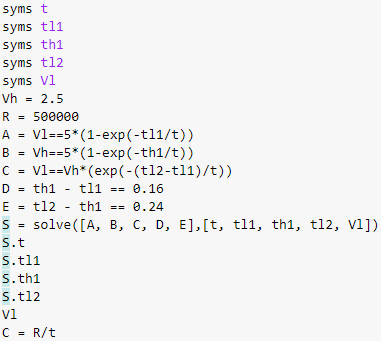
\includegraphics[width = 0.75\textwidth]{./Figures/script}